% Options for packages loaded elsewhere
\PassOptionsToPackage{unicode}{hyperref}
\PassOptionsToPackage{hyphens}{url}
\PassOptionsToPackage{dvipsnames,svgnames,x11names}{xcolor}
%
\documentclass[
  letterpaper,
  DIV=11,
  numbers=noendperiod]{scrartcl}

\usepackage{amsmath,amssymb}
\usepackage{iftex}
\ifPDFTeX
  \usepackage[T1]{fontenc}
  \usepackage[utf8]{inputenc}
  \usepackage{textcomp} % provide euro and other symbols
\else % if luatex or xetex
  \usepackage{unicode-math}
  \defaultfontfeatures{Scale=MatchLowercase}
  \defaultfontfeatures[\rmfamily]{Ligatures=TeX,Scale=1}
\fi
\usepackage{lmodern}
\ifPDFTeX\else  
    % xetex/luatex font selection
  \setmainfont[]{Times New Roman}
  \setsansfont[]{Times New Roman}
\fi
% Use upquote if available, for straight quotes in verbatim environments
\IfFileExists{upquote.sty}{\usepackage{upquote}}{}
\IfFileExists{microtype.sty}{% use microtype if available
  \usepackage[]{microtype}
  \UseMicrotypeSet[protrusion]{basicmath} % disable protrusion for tt fonts
}{}
\usepackage{xcolor}
\setlength{\emergencystretch}{3em} % prevent overfull lines
\setcounter{secnumdepth}{5}
% Make \paragraph and \subparagraph free-standing
\ifx\paragraph\undefined\else
  \let\oldparagraph\paragraph
  \renewcommand{\paragraph}[1]{\oldparagraph{#1}\mbox{}}
\fi
\ifx\subparagraph\undefined\else
  \let\oldsubparagraph\subparagraph
  \renewcommand{\subparagraph}[1]{\oldsubparagraph{#1}\mbox{}}
\fi


\providecommand{\tightlist}{%
  \setlength{\itemsep}{0pt}\setlength{\parskip}{0pt}}\usepackage{longtable,booktabs,array}
\usepackage{calc} % for calculating minipage widths
% Correct order of tables after \paragraph or \subparagraph
\usepackage{etoolbox}
\makeatletter
\patchcmd\longtable{\par}{\if@noskipsec\mbox{}\fi\par}{}{}
\makeatother
% Allow footnotes in longtable head/foot
\IfFileExists{footnotehyper.sty}{\usepackage{footnotehyper}}{\usepackage{footnote}}
\makesavenoteenv{longtable}
\usepackage{graphicx}
\makeatletter
\def\maxwidth{\ifdim\Gin@nat@width>\linewidth\linewidth\else\Gin@nat@width\fi}
\def\maxheight{\ifdim\Gin@nat@height>\textheight\textheight\else\Gin@nat@height\fi}
\makeatother
% Scale images if necessary, so that they will not overflow the page
% margins by default, and it is still possible to overwrite the defaults
% using explicit options in \includegraphics[width, height, ...]{}
\setkeys{Gin}{width=\maxwidth,height=\maxheight,keepaspectratio}
% Set default figure placement to htbp
\makeatletter
\def\fps@figure{htbp}
\makeatother

%\documentclass{article}

% todonotes package                          #####################

\usepackage[textsize=footnotesize]{todonotes}


%language                                    #####################

%\usepackage{times}
%\usepackage{t1enc}                               Trouble maker
%\usepackage[utf8x]{inputenc}
%\usepackage[polish]{babel}
%\usepackage{polski}


% math                                       #####################

%AMS
\usepackage{amsfonts}
\usepackage{amssymb}
\usepackage{amsthm}
\usepackage{amsmath}
\usepackage{mathtools}


% quote environment                        #######################  Unfortunately it destroys the font, only an issue in a mathmode

%\usepackage[T1]{fontenc} % Required for correct quotes with ""

%\renewenvironment{quote}
%{\list{}{\leftmargin=1em\rightmargin=1em}\item[]``}
%{''\endlist}

% spacing
\usepackage{setspace}
\onehalfspacing

% page geometry                              #####################


\usepackage{geometry}
 \geometry{a4paper,left=35mm,top=20mm,}

\setlength{\parindent}{10pt}
\setlength{\parskip}{1pt}

\usepackage{float}
\restylefloat{figure}

% abbreviations                              #####################

\newcommand{\ra}{\rangle}
\newcommand{\la}{\langle}
\newcommand{\n}{\neg}
\newcommand{\et}{\wedge}
\newcommand{\jt}{\rightarrow}
\newcommand{\ko}[1]{\forall  #1\,}
\newcommand{\ro}{\leftrightarrow}
\newcommand{\exi}[1]{\exists\, {_{#1}}}
\newcommand{\pr}[1]{\mathsf{P}(#1)}
\newcommand{\cost}{\mathsf{cost}}
\newcommand{\benefit}{\mathsf{benefit}}
\newcommand{\ut}{\mathsf{ut}}

\newcommand{\dkl}{D_{\mathsf{KL}}} % trying to add the definition of \dkl

\newcommand{\odds}{\mathsf{Odds}}
\newcommand{\ind}{\mathsf{Ind}}
\newcommand{\nf}[2]{\nicefrac{#1\,}{#2}}
\newcommand{\R}[1]{\texttt{#1}}
\newcommand{\prr}[1]{\mbox{$\mathtt{P}_{prior}(#1)$}}
\newcommand{\prp}[1]{\mbox{$\mathtt{P}_{posterior}(#1)$}}

\newcommand{\s}[1]{\mbox{$\mathsf{#1}$}}


\newtheorem{q}{\color{blue}Question}
\newtheorem{lemma}{Lemma}


\newtheorem{theorem}{Theorem}
\newtheorem{definition}{Definition}        % trying to add the def. environment



% bibliography                                #####################

%\usepackage[authoryear]{natbib}  % solution to the  natbib compilation error

%\bibliographystyle{apalike}





\KOMAoption{captions}{tableheading}
\makeatletter
\@ifpackageloaded{caption}{}{\usepackage{caption}}
\AtBeginDocument{%
\ifdefined\contentsname
  \renewcommand*\contentsname{Table of contents}
\else
  \newcommand\contentsname{Table of contents}
\fi
\ifdefined\listfigurename
  \renewcommand*\listfigurename{List of Figures}
\else
  \newcommand\listfigurename{List of Figures}
\fi
\ifdefined\listtablename
  \renewcommand*\listtablename{List of Tables}
\else
  \newcommand\listtablename{List of Tables}
\fi
\ifdefined\figurename
  \renewcommand*\figurename{Figure}
\else
  \newcommand\figurename{Figure}
\fi
\ifdefined\tablename
  \renewcommand*\tablename{Table}
\else
  \newcommand\tablename{Table}
\fi
}
\@ifpackageloaded{float}{}{\usepackage{float}}
\floatstyle{ruled}
\@ifundefined{c@chapter}{\newfloat{codelisting}{h}{lop}}{\newfloat{codelisting}{h}{lop}[chapter]}
\floatname{codelisting}{Listing}
\newcommand*\listoflistings{\listof{codelisting}{List of Listings}}
\makeatother
\makeatletter
\makeatother
\makeatletter
\@ifpackageloaded{caption}{}{\usepackage{caption}}
\@ifpackageloaded{subcaption}{}{\usepackage{subcaption}}
\makeatother
\ifLuaTeX
  \usepackage{selnolig}  % disable illegal ligatures
\fi
\usepackage{bookmark}

\IfFileExists{xurl.sty}{\usepackage{xurl}}{} % add URL line breaks if available
\urlstyle{same} % disable monospaced font for URLs
\hypersetup{
  pdftitle={Higher-order Probabilism},
  colorlinks=true,
  linkcolor={blue},
  filecolor={Maroon},
  citecolor={Blue},
  urlcolor={Blue},
  pdfcreator={LaTeX via pandoc}}

\title{Higher-order Probabilism}
\author{}
\date{2024-08-15}

\begin{document}
\maketitle

\begin{quote} \textbf{Abstract.}  Rational agents are often uncertain about the truth of many propositions. To represent this uncertainty, two options are typically on the table, precise and imprecise probabilism, but both fall short in some respect. Precise probabilism is not expressive enough, while imprecise probabilism suffers from belief inertia and the impossibility of proper scoring rules. We put forward a novel version of probabilism, higher-order probabilism, and we argue that it outperforms existing alternatives.

Keywords: Probabilism; Imprecise probabilities; Evidence; Probability; Belief inertia; Bayesian networks; Proper scores.

\end{quote}

\section{Introduction}\label{introduction}

\label{sec:introduction}

As rational agents, we are uncertain about the truth of many
propositions since our evidence is often fallible. To represent this
uncertainty, two options are typically on the table: precise and
imprecise probabilism. Precise probabilism models an agent's state of
uncertainty (or credal state) with a single probability measure: each
proposition is assigned a probability between 0 and 1 (a sharp
credence). The problem is that a single probability measure is not
expressive enough to distinguish between intuitively different states of
uncertainty (\S \ref{sec:precise-probabilism}). Alternatively, a
\emph{set} of probability measures can model an agent's uncertainty.
This approach, known as imprecise probabilism, does better than precise
probabilism in some respects but also runs into problems such as belief
inertia and the impossibility of defining proper scoring rules
(\S \ref{sec:imprecise-probabilism}).

To make progress, this paper argues that a rational agent's uncertainty
should be represented by a set of (higher-order) probability densities,
one for each (first-order) proposition of interest. The theory we
propose is not mathematically novel, nor are philosophers unfamiliar
with higher-order probabilities \textbf{CITE SOME: Skyrms, Gaifmann,
Domotor, Uchii, Pearl, Peijnenburg and Atkinson}. Here we address
specifically how our approach to higher-order probabilism can overcome
the problems of precise and imprecise probabilism
(\S \ref{sec:higher-order} and \S \ref{sec:proper-scores}). We also
argue that higher-order probabilism fares better when assessing the
probability of multiple propositions, dependent or independent
(\S \ref{sec:higher-order-conjunction} and
\ref{sec:higher-order-networks}). Many of the examples in this paper are
about coin tosses, but in the final two sections, we discuss legal
examples and illustrate the broader applicability of higher-order
probabilism.

\section{Precise probabilism}\label{precise-probabilism}

\label{sec:precise-probabilism}

Precise probabilism holds that a rational agent's uncertainty about a
proposition is to be represented as a single, precise probability
measure. Bayesian updating regulates how the prior probability measure
should change in light of new evidence that the agent learns. This is an
elegant and simple theory, but representing our uncertainty about a
proposition with a single, precise probability measure fails to capture
an important dimension of how our fallible beliefs reflect the evidence
we have (or have not) obtained. A couple of stylized examples featuring
coin tosses should make the point clear.

\begin{quote}
\textbf{No evidence v. fair coin}
You are about to toss a coin but have no evidence 
about its bias. You are completely ignorant. 
Compare this to the situation in which you know, 
based on overwhelming evidence, that the coin is fair. 
\end{quote}

\noindent On precise probabilism, both scenarios are represented by
assigning a probability of .5 to the proposition
\emph{the coin will land heads on the next toss} (or \emph{heads} for
short). If you are completely ignorant, the principle of insufficient
evidence suggests that you assign .5 to this proposition. Similarly, if
you are sure the coin is fair, assigning again .5 seems the best way to
quantify your uncertainty about the outcome. The agent's evidence in the
two scenarios is quite different, but the precise probability of
\emph{heads} cannot capture this difference.

\begin{quote}
\textbf{Learning from ignorance}
You toss a coin with unknown bias. You toss it 10 times and observe 5 heads. You toss it further and observe 50 heads in 100 tosses. 
\end{quote}

\noindent Since the coin initially had an unknown bias, you should
presumably assign a probability of .5 to the proposition \emph{heads},
if you stick with precise probabilism. After the 10 tosses, you again
assess the probability to be .5. You must have learned something, but
whatever that is, it is not reflected in the precise probability of
\emph{heads}. When you toss the coin 100 times and observe 50 heads, you
also learn something new, but your precise probability does not
change.\footnote{Another problem for precise probabilism is known as
  \emph{sweetening} {[}@sweetening2010{]}.}

These examples show that the precise probability of \emph{heads} is not
appropriately responsive to evidence. But instead of focusing on this
probability, the precise probabilist might respond that we should extend
the algebra and include propositions about the bias of the coin. As
evidence accumulates that the coin is fair, the (precise) probability of
the proposition \emph{the coin has a .5 bias} should go up, even though
the (precise) probability of \emph{heads} should remain .5. We think
this response is on the right track, but how does it generalize beyond
cases of coin tosses?

Suppose that, given a certain stock of evidence, \(A\) is more likely
than \(B\). Further, suppose that the acquisition of new evidence does
not change the probabilities. Admittedly, something has changed in the
agent's state of uncertainty: the quantity of evidence on which the
agent can assess whether \(A\) is more probable than \(B\) has become
larger. And yet, this change is not reflected in the precise
probabilities assigned to \(A\) and \(B\).\footnote{The distinction here
  is sometimes formulated in terms of the \emph{balance} of the evidence
  (that is, whether the evidence available tips in favor a hypothesis or
  another) as opposed to its \emph{weight} (that is, the overall
  quantity of evidence regardless of its balance); see
  @keynes1921treatise and @joyce2005probabilities.} The precise
probabilist might recommend we extend the algebra and include
propositions of the form
\emph{the probability of event X is such and such}. Since such
propositions contain a probability, assigning a probability to them
effectively amounts to using higher-order probabilities.\footnote{Interestingly,
  \textbf{PERAL ADD REFERENCE} argues that the semantics of higher-order
  probability statements can still be expressed in the language of
  first-order probability.} Our approach to higher-order probabilism
will not be quite that, for reasons we shall explain. Before going
higher-order, however, we should explore another view in the literature.

\section{Imprecise probabilism}\label{imprecise-probabilism}

\label{sec:imprecise-probabilism}

Imprecise probabilism holds that a rational agent's credal stance
towards a hypothesis is to be represented by a set of probability
measures, typically called a representor \(\mathbb{P}\), rather than a
single measure \(\mathsf{P}\). The representor should include all and
only those probability measures which are compatible with the evidence
(more on this point later).\footnote{For the development of imprecise
  probabilism, see @keynes1921treatise; @Levi1974ideterminate;
  @Gardenfors1982unreliable; @Kaplan1968decision;
  @joyce2005probabilities; @VanFraassen2006vague; @Sturgeon2008grain;
  @walley1991statistical. @bradley2019imprecise is a good source of
  further references. Imprecise probabilism is closely related to what
  we might call interval probabilism {[}@Kyburg1961;
  @kyburg2001uncertain{]}. In interval probabilism, precise
  probabilities are replaced by intervals of probabilities. Imprecise
  probabilism is more general since the representor set need not be an
  interval.} Modeling an agent's credal state by sets of probability
measures can easily accommodate the scenarios in the previous section
without adding propositions about coin biases. For instance, if an agent
is sure the coin is fair, their credal state would be represented by the
singleton set \(\{\mathsf{P}\}\), where \(\mathsf{P}\) is a probability
measure that assigns \(.5\) to \emph{heads}. If, on the other hand, the
agent knows nothing about the coin's bias, their credal state would be
represented by the set of all probabilistic measures, since none of them
is excluded by the available evidence.

So far so good. But now consider this scenario:

\begin{quote}
\textbf{Even v. uneven bias:}
 You have two coins and you are sure the probability of \emph{heads} is .4, if you toss one coin, and .6, if you toss the other. But you cannot tell which is which. You pick one coin at random and toss it.  Contrast this with an uneven case. You have four coins and you are sure three of them have bias $.4$ and one of them bias $.6$. You pick a coin at random and toss it. You should be three times more confident that the probability of getting heads is .4. rather than .6.
\end{quote}

\noindent The first scenario can be easily modeled by imprecise
probabilism. The representor would contain two probability measures; one
assigns .4. and the other assigns .6 to the proposition
\emph{the coin will land heads}. Yet imprecise probabilism cannot model
the second scenario. Since the probability measures in the set are all
compatible with the agent's evidence, no probability measure can be
assigned a greater (higher-order) probability than any other.\footnote{Other
  scenarios can be constructed in which imprecise probabilism fails to
  capture distinctive intuitions about evidence and uncertainty; see,
  for example, {[}@Rinard2013against{]}.}

These scenarios show that imprecise probabilism is not always expressive
enough. Worst still, imprecise probabilism suffers from three
shortcomings that do not affect precise probabilism: first, the idea of
compatibility between the available evidence and the probability
measures in the representator set is not clearly defined; second,
updating imprecise probabilities can run into belief inertia; and third,
no proper scoring rules exist for imprecise probabilities.

The first shortcoming has not received extensive discussion in the
literature. For imprecise probabilism, an agent's state of uncertainty
is represented by those probability measures that are \emph{compatible}
with the agent's evidence, but the notion of compatibility lacks a clear
definition in the literature. Roughly, think of it as the fact that the
agent's evidence does not outright rule out the probability measure in
question. The problem is that observations, evidence and data will
hardly rule out any probability measure. Admittedly, there will be
clear-cut cases: if you see the outcome of a coin toss is heads, you
reject the measure with \(\mathsf{P}(\emph{heads})=0\), and similarly
for tails. Another class of cases might arise while randomly drawing
objects from a finite set where the objective chances are
known.\footnote{Probability measures can be inconsistent with evidential
  constraints that agents believe to be true
  {[}@bradley2012scientific{]}, for example,
  \emph{structural constraints} such as ``\(X\) and \(Y\) are
  independent''. But, unless they come from an oracle, there will
  usually be some degree of uncertainty about the acceptability of these
  constraints.} But clear-cut cases aside, what else?

A second, related problem for imprecise probabilism is belief inertia
{[}@Levi1980enterprise{]}. Precise probabilism offers an elegant model
of learning from evidence: Bayesian updating. Imprecise probabilism, at
least \emph{prima facie}, offers an equally elegant model of learning
from evidence, richer and more nuanced. When faced with new evidence
\(E\) between time \(t_0\) and \(t_1\), the representor set should be
updated point-wise, running the standard Bayesian updating on each
probability measure in the representor:
\begin{align*} \label{eq:updateRepresentor}
\mathbb{P}_{t_1} = \{\mathsf{P}_{t_1}\vert \exists\, {\mathsf{P}_{t_0} \!\in  \mathbb{P}_{t_0}}\,\, \forall\, {H}\,\, \left[\mathsf{P}_{t_1}(H)=\mathsf{P}_{t_0}(H \vert E)\right] \}.
\end{align*}

\noindent Belief inertia arises in situations in which no amount of
evidence can lead the agent to change their initial belief state,
according to a given modeling strategy. Consider a situation in which
you start tossing a coin knowing nothing about its bias, so the range of
possibilities is \([0,1]\). After a few tosses, if you observed at least
one tail and one head, you can exclude the measures assigning 0 or 1 to
\emph{heads}. But else what can you learn? For any sequence of outcomes
that you can obtain and any probability value in \((0, 1),\) there will
exist a probability measure (conditional on the outcomes) that assigns
that probability to \emph{heads}. Consequently, the edges of your
resulting interval will remain the same.

Some downplay the problem of belief inertia and blame the uniform prior
{[}0, 1{]}.\footnote{Another strategy is to say that, in a state of
  ignorance, a special updating rule should be deployed
  {[}@Lee2017impreciseEpistemology{]}} Just as contingent propositions
should not be assigned (precise) probabilities of 0 or 1 since these
extreme values are unrevisable, by the same token the uniform prior
{[}0, 1{]} should not be used whenever it is impervious to revision
{[}@moss2020Imprecise{]}. More generally, it is unsurprising you will
not learn anything when you start from a place of ignorance
{[}@Joyce2010defense{]}. But, as we will see in the next section,
uniform priors are not necessarily unrevisable and can be a starting
point for learning. The problem lies with imprecise probabilities, not
with uniform priors as such.

The third problem for imprecise probabilism is to find suitable proper
scoring rules. In the precise case, scoring rules measure the distance
between a rational agent's probability measure and the actual value. The
Brier score is the most common scoring rule for precise
probabilities.\footnote{The Brier score is defined as the squared
  distance between the true state and the probability forecast, or
  formally, \((p(x)-V(x, w))^2\), where \(p(x)\) is the probability
  forecast and \(V(x, w)\) determines if a proposition obtains at \(w\)
  (\(V(x, w)=1\)) or not (\(V(x, w)=0\)). If, for example, the
  proposition `rain' obtains at \(w\), the forecast `rain with .9
  probability' would be more accurate at \(w\) than the forecast `rain
  with .8 probability'. If, on the other hand, the proposition `not
  rain' obtained at \(w\), the latter forecast would be more accurate.}
A requirement of scoring rules is \emph{propriety}: any rational agent
will expect their probability measure to be more accurate than any
other. A bit more formally, the expected inaccuracy of \(p\) from the
perspective of \(p\) should always be smaller than the expected
inaccuracy of \(p\) from the perspective of another distribution \(q\).
After all, if an agent thought a different probability measure was more
accurate, they should switch to it. Well-known results demonstrate the
strict propriety of the Brier score for precise
probabilities.\footnote{Besides propriety, other common requirements
  (which the Brier score also satisfies) are: the score \(I(p, w)\)
  should be a function of the probability distribution \(p\) and the
  true state \(w\) (extensionality); and the score should be a
  continuous function around \(p\) (continuity).} Can similar results be
established for imprecise probabilities? The answer is likely to be
negative.

In the precise case, let \(I(p, w)\) be an inaccuracy score of a
probability distribution \(p\) relative to the true state \(w\). Its
expected inaccuracy, from the perspective of \(p\) equals
\[\sum_{w \in W}p(w)I(p, w).\] \noindent In the imprecise case, let
\(I([p_-, p_+], w)\) be the inaccuracy score for the interval
\([p_-, p_+]\). What is its expected inaccuracy from the perspective of,
say, the interval \([p_-, p_+]\) itself? There is no straightforward
answer to this question because \(I([p_-, p_+], w)\) cannot be
multiplied by \([p_-, p_+]\), in the way in which \(I(p, w)\) can be
multiplied by \(p(w)\). The expected inaccuracy of \([p_-, p_+]\) can be
evaluated from the perspective of the precise probabilities at its
edges.\footnote{So the expected inaccuracy would equal
  \(\sum_{w\in W} p_-(w)I([p_-, p_+], w)\) or
  \(\sum_{w\in W} p_+(w)I([p_-, p_+], w).\)} The problem is that, in
this case, finding a proper inaccuracy score that is also continuous is
mathematically impossible {[}@seidenfeld2012forecasting{]}.

Proper scoring rules are often used to formulate accuracy-based
arguments for precise probabilism. These arguments show (roughly) that,
if your precise measure follows the axioms of probability theory, no
other non-probabilistic measure is going to be more accurate than yours
whatever the facts are. But, without proper scoring rules for imprecise
probabilities, the prospects for an accuracy-based argument for
imprecise probabilism look dim {[}@Mayo-Wilson2016scoring;
@CampbellMoore2020accuracy{]}.\footnote{Moreover, as shown by
  @Schoenfield2017accuracy, if an accuracy measure satisfies certain
  plausible formal constraints, it will never strictly recommend an
  imprecise stance, as for any imprecise stance there will be a precise
  one with at least the same accuracy.}

\section{Higher-order probabilism}\label{higher-order-probabilism}

\label{sec:higher-order}

Let us take stock. Imprecise probabilism is expressive enough to model
the difference between a state in which there is no evidence about a
proposition (or its negation) and a state in which the evidence for and
against a proposition is in equipoise. However, imprecise probabilism
has its own expressive limitations, for example, it cannot model the
case of uneven bias. In addition, imprecise probabilism faces
difficulties that do not affect precise probabilism: the notion of
compatibility between a probability measure and the evidence is too
permissive; belief inertia makes it impossible for a rational agent to
learn via Bayesian updating; and no proper scoring rules exist for
imprecise probabilism. We will now show that higher-order probabilism
overcomes the expressive limitations of imprecise probabilism without
falling prey to these difficulties.

Proponents of imprecise probabilism already hinted at the need to rely
on higher-order probabilities. For instance, @bradley2012scientific
compares the measures in a representor to committee members, each voting
on a particular issue, say the true chance or bias of a coin. As they
acquire more evidence, the committee members will often converge on a
chance hypothesis. But such convergence up cannot be modeled by
imprecise probabilism alone: a probability distribution over chance
hypotheses is needed.\footnote{In a similar vein,
  @joyce2005probabilities, in a paper defending imprecise probabilism,
  explicates the notion of weight of evidence using a probability
  distribution over chance hypotheses.} That one should use higher-order
probabilities has also been suggested by critics of imprecise
probabilism. @Carr2020impreciseEvidence argues that sometimes evidence
requires uncertainty about what credences to have. Carr, however, does
not develop this suggestion formally, and does not explain how her
approach would fare against the difficulties affecting imprecise
probabilism. We now set out to do precisely that.

The central idea of our approach to higher-order probabilism is this:
instead of a probability between 0 and 1, rational agents assign a
probability density to each proposition of interest. For example,
consider the scenario in which the agent is about to toss a coin whose
known bias is either .4 or .6, but the former is three times more
likely. This scenario---which imprecise probabilism cannot model---can
be easily modeled within high-order probabilism. The proposition
\emph{the coin will land heads on the next toss} is assigned a
probability density whose mass is 3/4 on the .4 value and the remaining
1/4 on the .6 value, as illustrated in
Figure~\ref{fig-evidenceResponse}. To be sure, an agent's uncertainty
about a proposition could---perhaps, should---sometimes be represented
by a single probability value. Higher-order probabilism does not
prohibit that. There may well be cases in which an agent's uncertainty
is aptly represented by the expectation, usually defined as
\(\int_{0}^{1} p f(p) \, dp\), where \(p\) is the first-order
probability of a given proposition and \(f\) is the density representing
the agent's uncertainty about \(p\). But this need not always be the
case. If the probability distribution is not sufficiently concentrated
around a single value, a one-point summary will fail to do justice to
the nuances of the agent's credal state.\footnote{In the case of uneven
  biases, for example, representing the agent's credal state with the
  expectation \(.75 \times .4 + .25 \times .6 = .45\) would fail to
  capture the agent's different epistemic attitudes towards the two
  biases. The agent believes the two biases have different
  probabilities, and is also certain the bias is \emph{not} .45.}

So, an agent's state of uncertainty (or credal stance) towards a
proposition \(\mathbf{x}\) is not represented by a probability value
\(p(\mathbf{x})\) between 0 and 1, but by a probability density
\(f_\mathbf{x}(p(\mathbf{x}))\), where the first-order probability
\(p(\mathbf{x})\) is the parameter in question and is treated as a
random variable. (For computational ease, we will use a higher-order
discretized density ranging over 1000 first-order probabilities.) More
generally, let \(\mathbf{X}\) be the set of first-order propositions an
agent is interested in (more on this restriction soon). For each
proposition \(\mathbf{x}\in\mathbf{X}\), the rational agent will assign
a probability density \(f_\mathbf{x}(p(\mathbf{x}))\), and not simply a
probability value \(p(\mathbf{x})\). The mapping from propositions to
densities models the agent's overall state of uncertainty.\footnote{This
  approach lines up with common practice in Bayesian statistics, where
  the primary role of uncertainty representation is assigned to the
  whole distribution. Summaries such as the mean, mode standard
  deviation, mean absolute deviation or highest posterior density
  intervals are only succinct ways of representing uncertainty.}

\begin{figure}[t]

\centering{

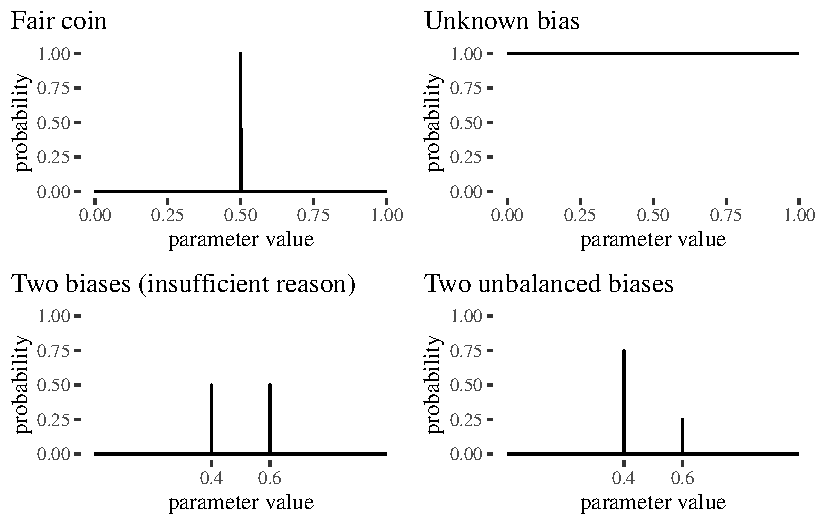
\includegraphics[width=0.65\textwidth,height=\textheight]{imp_philosophical_agust2024_files/figure-pdf/fig-evidenceResponse-1.pdf}

}

\caption{\label{fig-evidenceResponse}Examples of higher-order
distributions for a few scenarios problematic for both precise and
imprecise probabilism.}

\end{figure}%

Besides its greater expressive power in modeling uncertainty,
higher-order probabilism does not fall prey to the technical
difficulties of imprecise probabilism. It does not fall prey to belief
inertia. Consider a situation in which you have no idea about the bias
of a coin. You start with a uniform distribution over \([0,1]\) as your
prior. Observing any non-zero number of heads will exclude 0 and
observing any non-zero number of tails will exclude 1 from the basis of
the posterior. The posterior distribution will become more centered as
the observations come in. This result is a straightforward application
of Bayesian updating. Instead of plugging sharp probability values into
the formula for Bayes's theorem, the factors to be multiplied in the
theorem are probability densities (or ratios of densities).
Figure~\ref{fig-intertia2} illustrates---starting with a uniform
distribution---how the posterior distribution changes after successive
observations.\footnote{Assuming independence and constant probability
  for all the observations, learning is modeled the Bayesian way. You
  start with some prior density \(p\) over the parameter values. If you
  start with a complete lack of information, \(p\) should be uniform.
  Then, you observe the data \(D\) which is the number of successes
  \(s\) in a certain number of observations \(n\). For each particular
  possible value \(\theta\) of the parameter, the probability of \(D\)
  conditional on \(\theta\) follows the binomial distribution. The
  probability of \(D\) is obtained by integration. That is:
  \begin{align*}
  p(\theta \vert D) & = \frac{p(D\vert \theta)p(\theta)}{p(D)}\\
  & = \frac{\theta^s (1-\theta)^{(n - s)}p(\theta)}{\int (\theta')^s (1-\theta')^{(n - s)}p(\theta')\,\, d\theta'}.
  \end{align*}}

\begin{figure}

\centering{

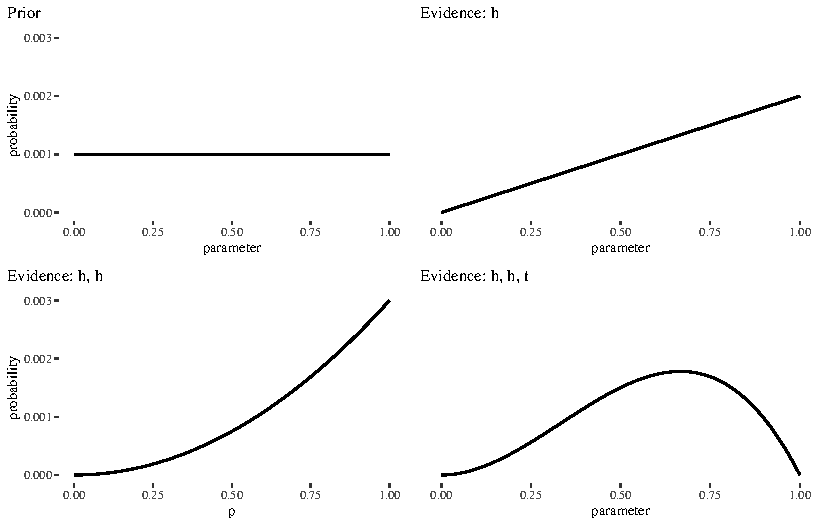
\includegraphics[width=0.75\textwidth,height=\textheight]{imp_philosophical_agust2024_files/figure-pdf/fig-intertia2-1.pdf}

}

\caption{\label{fig-intertia2}As observations of heads, heads and tails
come in, extreme parameter values drop out of the picture and the
posterior is shaped by the evidence.}

\end{figure}%

The impossibility of defining proper scoring rules was another weakness
of imprecise probabilism. This is a significant shortcoming, especially
because proper scores do exist for precise probabilism. Fortunately, one
can show that there exist proper scoring rules for higher-order
probabilism. We defend this claim in greater detail in the next section.
But before turning to this topic, we will discuss an alternative
approach to higher-order probabilism.

As noted earlier, the set \(\mathbf{X}\) of propositions of interest is
restricted to first-order ones. We are here relying on the intuitive
distinction between propositions more directly about events in the
world, such as \emph{the coin will land heads on the next toss}, and
more abstract constructs such as the probabilities of these
propositions. Only the former are included in the set \(\mathbf{X}\).
Now, the precise probabilist might agree with this distinction but
insist that going higher-order in the way we are suggesting is
unnecessary. After all, the set of propositions of interest need not be
limited to first-order ones. It can be extended to include second-order
propositions, those about the probabilities of first-order propositions.
Then, an agent's state of uncertainty can be modeled by a single,
precise probability measure defined over all members of this extended
set denoted by \(\mathbf{X}^2\). The scenario of uneven coins would not
pose a problem, since the (second-order) propositions about the coin
biases can be assigned different (precise) probabilities, that is,
\(p(\emph{bias}=.4)=3/4\) and \(p(\emph{bias}=.6)=1/4\). Call this
approach \(\mathbf{X}^2\)-precise probabilism to distinguish it from the
simpler version of precise probabilism.

On \(\mathbf{X}^2\)-precise probabilism, the agent is expected to have
attitudes towards uncountably many propositions of the form
\(\emph{bias}=x\). This approach might be viable, but it is in no way
simpler than higher-order probabilism. For consider the (first-order)
proposition \emph{the coin will land heads on the next toss} (in short,
\emph{heads}) and the (second-order) \emph{the coin has a bias of .5}.
We expect them to be related in precise ways, for example, it is
inconsistent to assign a probability of one (or an extremely high or low
probability) to both of them. Evidently, the two propositions are not
probabilistically independent, but their dependence is conceptual, not
empirical: that a coin is fair just means that its probability of
landing heads cannot be extremely high. Higher-order probabilism can
easily model this conceptual dependence by positing that the expectation
of the (higher-order) density \(f_{\emph{heads}}(p(\emph{heads}))\)
should equal the (first-order) probability \(p(\emph{heads})\). Instead,
\(\mathbf{X}^2\)-precie probabilism will have to hard code (infinitely
many!) dependencies between first- and second-order propositions as
\textit{ad hoc} postulates.

Besides its greater simplicity, another advantage of our higher-order
approach is that, at the technical level, it is by no means novel.
Bayesian probabilistic programming languages embrace the well-known idea
that parameters can be stacked and depend on each other
{[}@Bingham2021PPwithoutTears{]}. But, while the technical machinery has
been around for a while, it has not been deployed by philosophers to
model a rational agent's uncertainty or credal state.\footnote{Our
  approach to higher-order probabilism should also be distinguished from
  what we might call higher-order (imprecise) probabilism. On this
  account, an agent's state of uncertainty is modeled by a set of
  probability measures defined over a fixed algebra of first-order
  propositions (just like imprecise probabilism does), and in addition,
  a probability distribution over those first-order probability
  measures. This is a generalization of imprecise probabilism.}

\section{Higher-order proper scores -- !STILL NEDS
REVISIONS!}\label{higher-order-proper-scores-still-neds-revisions}

\label{sec:proper-scores}

Despite the difficulties that plague imprecise probabilism in defining
proper scoring rules, here we put forward an intuitively plausible
scoring rule for higher-order probabilities that is both proper and
continuous. Building on existing work on this topic
(@HersbachDecomp2000, @Pettigrew2012Epistemic-Utili, @GneitRafter2007),
we begin by laying out two common measures of distance between
probabilities distributions. We then use these measures to define
higher-order inaccuracy scores and argue for their propriety.

As a measure of the distance between two distributions \(p\) and \(q\),
the Cramer-Von-Mises (CM) measure is a natural starting point. It is
defined as follows: \begin{align*}
D_{\text{CM}}(p,q) & = \sum_{x} \vert P(x) - Q(x)\vert^2, 
\end{align*} \noindent where \(x\) ranges over all hypotheses under
consideration (i.e.~the elements of the sample space). The CM measure
sums over the square of the differences between \(P(x)\) and \(Q(x)\)
for each value \(x\), where \(P\) and \(Q\) are the cumulative
distributions corresponding to the probability distribution \(p\) and
\(q\). Looking at cumulative densities is a technical requirement that
ensures that all densities are considered on the same scale. As an
alternative measure, the Kullback-Leibler (KL) divergence is a common
information-theoretic measure of distance between probability
distributions. The distance between \(p\) and \(q\) from the perspective
of \(p\) is defined as follows:
\[ D_{\text{KL}}(p || q) = \sum_{x} p(x) \log\left(\frac{p(x)}{q(x)}\right) \]
\noindent The KL measure sums over the log of the ratio of \(p(x)\) to
\(q(x)\) for each value \(x\). Note that the KL measure contains a
weighing by the distributions \(p\), while the CM measure does not. For
ease of computation, these two measures are discretized.\footnote{In the
  continuous case, KL divergence is defined as the differential KL
  divergence and the CM measure as the area under the squared Euclidean
  distances between the corresponding cumulative density functions. That
  is, \(D_{CM}(p,q)  = \int_{0}^{1} \vert P(x) - Q(x)\vert^2 \, dx\).
  There are no readily computable solutions to this integral, although
  it can sometimes be evaluated in the closed form {[}@GneitRafter2007,
  p. 366{]}.}

Both measures can be turned into inaccuracy scores provided one of the
two distributions plays the role of the higher-order distribution whose
accuracy is to be measured and the other distribution tracks the true
state of the world. But before moving forward, some notation is needed.
Since many of the examples in this paper are about coin tosses and their
biases, let \(\theta_1, \dots, \theta_n\) be a finite set of hypotheses
about the bias of a coin (this is our discretization of the sample
space). Depending on the state of the world, one of these hypotheses
will correspond to the true coin bias, call it \(\theta_k\). Each
\(\theta_k\) is paired with an omniscient distribution \(Ind^k(\cdot)\),
such that \(Ind^k(\theta_i)\) is 1 if \(i=k\) and \(0\) otherwise. In
other words, since the omniscient distribution tracks the true state of
the world (i.e.~the true bias being \(\theta_k\)), it will assign 1 to
the true chance hypothesis \(\theta_k\) and 0 to all the others. For
simplicity, we will write \(Ind^k_i\) instead of \(Ind^k(\theta_i)\).

With this notation in place, the inaccuracy of a higher-order
probability distribution \(p\) if the true state is \(\theta_k\) can be
defined using the CM measure, as follows: \begin{align*}
I_{\text{CM}}(p, \theta_{k}) &= \sum_{i=1}^n \vert \mathsf{P}(\theta_i) - Ind^k_i \vert ^2 
\end{align*}

\noindent Using instead KL divergence between \(p\) and \(Ind^k\), the
inaccuracy of a higher-order probability distribution \(p\) if the true
state is \(\theta_k\) can be defined, as follows: \begin{align*}
I_{\text{KL}}(p, \theta_k)  = \sum_{i=1}^n Ind^k_i \log\left(\frac{Ind^k_i}{p(\theta_i)}\right)
\end{align*}

\noindent As shown in the appendix, \(I_{\text{KL}}(p, \theta_k)\) boils
down to \(-\log p(\theta_k)\). If, for example, the true bias of the
coin is \(.6\) and the higher-order distribution \(p\) assigns \(.8\) to
this bias, the higher-order inaccuracy score of \(p\) would be
\(-\log (.8)\).\footnote{On this approach, two distributions \(p\) and
  \(p'\) which assign the same probability to the true coin bias will
  have the same inaccuracy score even though they might differ in the
  probabilities they assign to other possible coin biases. So the shape
  of the distribution does not matter for the inaccuracy score, but it
  does matter for expected inaccuracy (more on this soon).}

To check that the inaccuracy scores just defined work as intended,
consider a variation of a scenario by @Schoenfield2017accuracy. A
rational agent is invited to engage in a bet by an opponent who has a
representative bag of coins coming from a factory where the distribution
of bias among the coins produced, the true generative process, is known.
It is a mixture of two normal distributions centered at \(.3\) and at
\(.5\), both with a standard deviation of \(.05\). The opponent randomly
selects one of the coins in the bag and flips it. The rational agent who
knows this set-up may form a number of higher-order credal states in
response to this information. Consider three such credal states, out of
many options: first, a faithful bimodal distribution centered at \(.3\)
and \(.5\); second, a unimodal distribution centered at \(.4\); third, a
wide bimodal distribution centered at \(.2\) and \(.6\). The three
options are depicted in Figure~\ref{fig-emc}. All of them have expected
values at about \(.4\). So, if precise probabilities were the only
measure of uncertainty, \(.4\) would be the most natural value to assign
to the probability that coin came up, say, heads. The three
distributions, however, differ in how they represent higher-order
uncertainty, and it seems that the faithful bimodal distribution gives
the best representation, a point to which we will return.

\begin{figure}[H]

\centering{

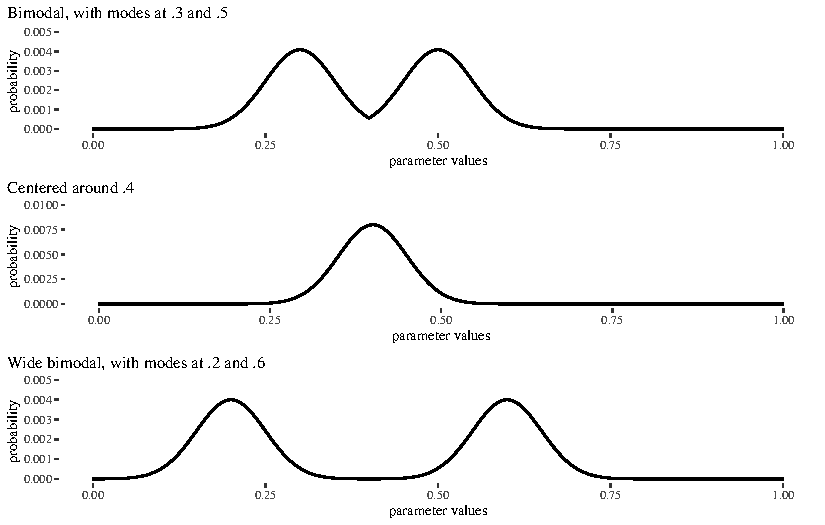
\includegraphics[width=0.7\textwidth,height=\textheight]{imp_philosophical_agust2024_files/figure-pdf/fig-emc-1.pdf}

}

\caption{\label{fig-emc}Three distributions in a vague EMS scenario. The
distributions are built from normal distributions with standard
deviation \(.05\), the bimodal ones are joint in the middle. All of them
have expected values \(\approx .4\).}

\end{figure}%

\begin{figure}[H]

\centering{

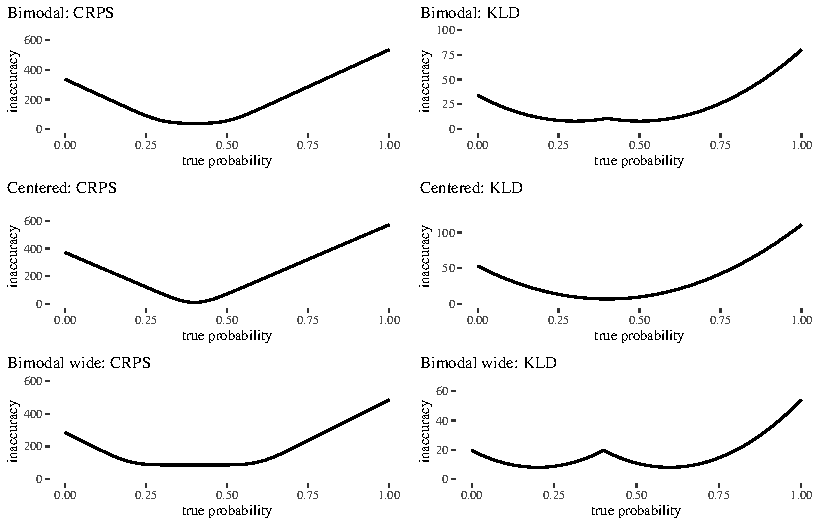
\includegraphics[width=0.7\textwidth,height=\textheight]{imp_philosophical_agust2024_files/figure-pdf/fig-inaccuracies2-1.pdf}

}

\caption{\label{fig-inaccuracies2}CM and KL divergence based
inaccuracies relative to \(n\) true chance hypotheses for the three
distributions, faithful bimodal, centered unimodal and wide bimodal.}

\end{figure}%

The accuracy scores of these higher-order distributions are in
Figure~\ref{fig-inaccuracies2}. Each point in the graph reflects the
accuracy score calculated relative to a possible omniscient distribution
corresponding to the values of \(\theta\), the true bias of the coin.
Both inaccuracy scores behave as intended. The inaccuracy scores are
higher at the extremes: if the true coin bias is indeed close to 1 (the
coin is weighted to heads) or 0 (the coin is weighted to tails), the
three distributions consider these biases extremely unlikely. However,
an important difference transpires between the CR and KL measures. For
chance hypotheses between the peaks of the two bimodal distributions,
the CR measure remains flat, an artifice of using a squared distance
metric. By contrast, the KL-based inaccuracy score jumps slightly for
values in between the peaks. This outcome is more intuitive, and a
reason to prefer KL-based inaccuracy scores.

To complete our discussion, the final step is argue for the propriety of
the scoring rules \(I_{KL}\) and \(I_{CM}\). The higher-order score
\(I(p, \theta_k)\), whether in the KL or CM version, is strictly proper
if, for any other probability distribution \(q\) different from \(p\),
the following holds:

\[ \sum_{k=1}^n  p(\theta_k) I(p, \theta_k) < \sum_{k=1}^n  q(\theta_k)I(p, \theta_k).\]

\noindent That is, the expected inaccuracy of \(p\) must be lower when
evaluated from the perspective of itself compared to any other
distribution \(q\). That the inequality holds is confirmed by
simulations in our running example. The expected inaccuracies, in the KL
and CM versions, of the three distributions---faithful bimodal, wide
bimodal and unimodal---from their own perspective, as well as from the
perspective of the other distributions, are in
\mbox{Table \ref{tbl:expected2}.} The results show that from their own
perspective, the distributions see themselves as the least inaccurate.

\begin{small}
\begin{table}[H]
\begin{tabular}{lrrrrrr}
& \multicolumn{3}{c}{CM} & \multicolumn{3}{c}{KL} \\
\toprule
  & bimodal & centered & wide bimodal & bimodal & centered & wide bimodal\\
\midrule
bimodal & 64.670 & 78.145 & 88.380 & 8.577 & 10.655 & 11.336\\
centered & 41.657 & 28.181 & 85.911 & 9.239 & 7.690 & 15.627\\
wide bimodal & 137.699 & 171.719 & 113.989 & 11.541 & 19.231 & 8.689\\
\bottomrule
\end{tabular}
\caption{Expected inaccuracies of the three distributions from their own perspective and that of the other distributions. Each row corresponds to a perspective.}
\label{tbl:expected2}
\end{table}
\end{small}

\noindent To generalize this argument, we prove the strict propriety of
the KL-based inaccuracy measure in the appendix. The gist of the proof
is this: the expected KL-based inaccuracy of \(p\) from the perspective
of \(p\) itself equals the entropy of \(p\), denoted by \(H(p)\), while
the expected inaccuracy of \(p\) from the perspective of a different
distribution \(q\) equals the cross-entropy \(H(p, q)\). Since
\(H(p) < H(p, q)\) always holds by Gibb's inequality when \(p\neq q\),
the KL-based inaccuracy of a distribution from its own perspective will
always be the lowest.

A corollary of the propriety of the KL- or CM-based scoring rules is
that the faithful bimodal distribution should be preferred over the
others. The unimodal distribution, while centering on the expected
value, gets the chances wrong, and the wide bimodal has its guesses too
close to the true values and too far from the known chances. So the
faithful bimodal seems the most evidence-responsive. How can this
intuition be captured formally? The expected inaccuracy of each
distribution should be measured from the perspective of the true
generative process, which we know to be the faithful bimodal centered at
.3 and .5. By strict propriety, the expected inaccuracy of the faithful
bimodal is the lowest, a good reason to prefer it over the
others.\footnote{Alternatively, note that the KL-distance or CM-distance
  between the faithful bimodal distribution and the true generative
  process (which is the faithful bimodal itself), is by definition zero,
  while it is greater than zero for the other distributions. So, again,
  the faithful bimodal should be preferred.}

\section{Conjunctions - !STILL NEEDS
REVISIONS!}\label{conjunctions---still-needs-revisions}

\label{sec:higher-order-conjunction}

Here is where we are. We have seen that imprecise probabilities model
uncertainty better than precise ones. But imprecise probabilities fall
short in their own way, for example, when the biases of a coin are not
equally likely given the evidence available. Higher-order probabilities
are better able to model these more complex scenarios. They also avoid
the pitfalls of imprecise probabilities, such as belief inertia and the
difficulty of finding proper scoring rules.

One limitation of the discussion so far, however, is that we only looked
at assessing probabilities of individual events, say whether a coin
would come up heads or tails. But, of course, rational agents may need
to assign probabilities to multiple events, for example, the conjunction
of two events. Suppose I am holding two coins, and I have information
about their respective biases. What is, then, the probability that they
both come up, say, heads? In the precise case, the answer is
straightforward: assuming independence, it is enough to multiply the
individual probabilities. But what happens in the imprecise case? And
how to proceed with higher-order probabilities? Once again, we will see
that in assessing probabilities for conjunctions of events higher-order
probabilities fare better than precise and imprecise ones.

Instead of relying on coin tosses, we will go through a legal example.
We selected this example to illustrate how higher-order probabilities
can be useful beyond cases of coin tossing. In a murder case, the police
recover two items of so-called match evidence: first, hair found at the
crime scene matches the defendant's hair; and second, the fur of the
defendant's dog matches the fur found in a carpet wrapped around one of
the bodies.\footnote{The hair evidence and the dog fur evidence are
  stylized after two items of evidence in the notorious 1981 Wayne
  Williams case {[}@deadman1984fiber1; @deadman1984fiber2{]}.} These two
matches constitute evidence against the defendant. The most obvious
explanation is that the defendant visited the crime scene and
contributed both traces. The alternative explanation is that the matches
are a coincidence. Maybe another person visited the scene and happened
to have the same hair type and a dog with the same fur type. How likely
is that? Trial experts usually provide coincidental match probabilities
(also called random match probabilities). They express the likelihood
that, by coincidence, a random person (or a random dog) who is not a
contributor would still match. If the coincidental match probabilities
are low, the two matches would be strong incriminating evidence. If they
are not low---the hair type and dog fur type are common---the two
matches would be weak incriminating evidence.

It is customary to rely on database frequencies to assess the
coincidental match probabilities, for example, by counting how many
matches are found in a sample of the human population or the canine
population. Suppose the matching hair type occurs 0.0253 times in a
reference database, and the matching dog fur type occurs 0.0256 times in
a reference database (more on how these numbers are calculated soon).
These frequencies give the individual coincidental probabilities. To
assess the probability of the two coincidental matches happening
jointly, it is enough to multiply the individual probabilities: 0.0253
\times  0.0256 = \ensuremath{6.48\times 10^{-4}}. Multiplication is
allowed on the assumption that the coincidental matches are independent
events.\footnote{The two matches are independent conditional on the
  hypothesis that the defendant is not a contributor.} The resulting
joint probability is very small. The two matches, combined, are strong
evidence against the defendant, or so it would appear.

This is the story told by the precise probabilist. But this story misses
something crucial. As it happens, the coincidental match probability for
hair evidence is based on \(29\) matches found in a sample database of
size \(1,148\), while the coincidental match probability for the dog
evidence is based on finding \(2\) matches in a smaller database of size
\(78\). The relative frequencies are about \(.025\) in both cases, but
the two samples differ in size. The smaller the sample, the greater the
uncertainty about the match probabilities. So, for individual pieces of
evidence, simply reporting the exact numbers makes it seem as though the
evidential value of the hair and fur matches is the same, but actually,
it is not.\footnote{The probabilities in the Wayne Williams case on
  which our running example is based were \(1/100\) for the dog fur, and
  \(29/1148\) for Wayne Williams' hair. Probabilities have been slightly
  but not unrealistically modified to be closer to each other in order
  to make a conceptual point: the same first-order probabilities, even
  when they sound precise, may come with different degrees of
  second-order uncertainty.} In the aggregate, multiplying the
coincidental match probabilities further washes away this difference.

A better approach is available: take into account higher-order
uncertainty. Figure~\ref{fig-densities} (upper part) depicts
higher-order probability distributions of different coincidental match
probabilities given the sample data---the actual number of matches found
in the sample databases. As expected, some coincidental probabilities
are more likely than others, and since the sizes of the two databases
are different, the distributions have different spreads: the smaller the
database the greater the spread, the greater the uncertainty about the
coincidental probability. In light of this, Figure~\ref{fig-densities}
(lower part) depicts the probability distribution for the joint
coincidental match probabilities associated with both hair and fur
evidence. The mathematics here is straightforward: once the higher-order
distributions are known, simply multiply them to obtain the higher-order
distribution of the joint coincidental match probabilities.

\begin{figure}[H]

\centering{

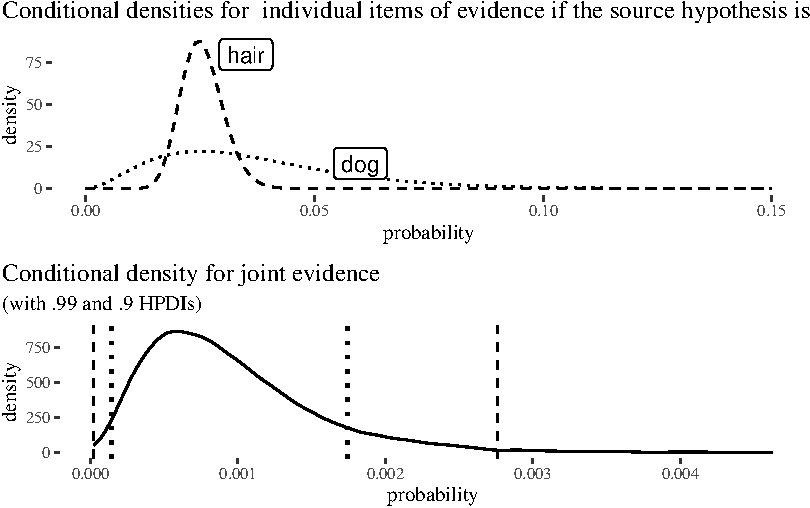
\includegraphics[width=0.8\textwidth,height=\textheight]{imp_philosophical_agust2024_files/figure-pdf/fig-densities-1.pdf}

}

\caption{\label{fig-densities}Beta densities for individual items of
evidence and the resulting joint density with .99 and .9 highest
posterior density intervals, assuming the sample sizes as discussed and
independence, with uniform priors.}

\end{figure}%

The precise probabilist might insist that our best assessment of the
first-order coincidental match probabilities is still the relative
frequency of matches found in the database, whether large or small. All
things considered, our best assessment of the match probabilities for
both fur and hair evidence should be about \(.025\), based on the
relative frequencies 2/78 and 29/1,148. After all, if we were to bet
whether a dog or a human picked at random would have the matching fur or
hair type, our odds should be \(.025\) no matter the size of the
database. This argument has some bite for individual events. In fact,
the expected values of the coincidental probabilities for hair and match
evidence---based on the higher-order distributions in
Figure~\ref{fig-densities} (upper part)---still end up being about
\(.025\). If, as the precise probabilist assumes, first-order
probabilities are all we should care about, going higher-order would
seem a needless complication.

This line of reasoning, however, breaks down when evaluating
conjunctions of events. What should our betting odds be for the
proposition that a human and a dog, both picked at random, would have
the matching fur and hair type in question? For the precise probabilist,
the answer is straightforward: on the assumption of independence,
multiply the \(.025\) individual match probabilities and obtain a joint
match probability of \ensuremath{6.48\times 10^{-4}}. The higher-order
probabilist will proceed differently. In assessing first-order match
probabilities, they will retain information about higher-order
uncertainty as much as possible. This can done in two steps: first,
aggregate the higher-order distributions for the two-match probabilities
and obtain a higher-order distribution for the joint match probability
(see Figure~\ref{fig-densities}); next, to obtain our best assessment of
the first-order joint match probability, take the expected value of this
latter distribution. Interestingly, the higher-order probabilist will
assign \ensuremath{9.38\times 10^{-4}} to the joint coincidental match
probability, a value greater than what the precise probabilist would
assign.

So, the higher-order and precise probabilist will disagree about the
betting odds for the proposition that a human and a dog, both picked at
random, would have the matching fur and hair type in question. The
disagreement will become even starker as a larger number of independent
items of evidence are evaluated.\footnote{Consider the simple case of
  independent items of evidence whose individual match probabilities are
  \(.025\). For three, five and seven items of evidence, the joint match
  probabilities would be: \ensuremath{1.25\times 10^{-4}},
  \ensuremath{3\times 10^{-7}} and \ensuremath{8\times 10^{-10}} (for
  the precise probabilist); \ensuremath{5.34\times 10^{-4}},
  \ensuremath{1.68\times 10^{-5}} and \ensuremath{9.999\times 10^{-7}}
  (for the higher-order probabilist, based on small databases of size
  20); and \ensuremath{1.08\times 10^{-4}}, \ensuremath{2\times 10^{-7}}
  and \ensuremath{6\times 10^{-10}} (for the higher-order probabilist,
  based on larger databases of size 20,000).} Who should be trusted?
Since the higher-order probabilist takes into account more
information---that is, information about the strength of evidence as
reflected in sample size---there is good reason to think that the
higher-order probabilist should be trusted more than the precise
probabilist.

We have not considered yet how imprecise probabilism fares in assessing
the probabilities of multiple events in conjunction. Recall that the
probability measures in the representor set are those compatible with
the evidence. Now, almost any coincidental match probability will be
compatible with any sample data. Think by analogy to coin tossing: even
a coin that has a .99 bias toward tails could come up heads on every
toss. This series of outcomes is unlikely but possible. Similarly, a
hair type that has a match probability extremely small could still be
found several times in a sample population. So the appropriate interval
would be {[}0,1{]} for both coincidental match probabilities, and the
same for the conjunction. This result would make it impossible to learn
anything. So this route is a non-starter.

Suppose instead we rely on reasonable ranges of coincidental match
probabilities, for example, (.015,.037) (.002, .103), for hair and fur
match evidence respectively.\footnote{These are 99\% credible intervals
  using uniform priors. A 99\% credible interval is the narrowest
  interval to which the expert thinks the true parameter belongs with
  probability .99. On credible intervals, see @kruschke2015doing.} As
expected, the range is set wider for dog fur match evidence than hair
match evidence: the uncertainty about the dog fur match probability is
greater since the sample database was smaller. This is a good feature of
the interval approach, unavailable to the precise probabilist. But how
to assess the joint uncertainty? The most natural strategy is to focus
on what happens at the edges of the two intervals. Reasoning with
representor members at the edges of the intervals will yield the most
extreme probability measure the impreciser is committed to, the
worst-case and best-case scenarios. Following this strategy yields a new
range for the joint match probabilities: (.00003, .003811).\footnote{Redoing
  the calculations using the upper bounds of the two intervals yields
  \(.037 \times .103 =.003811\). This number is around 5.88 times
  greater than the original, precise estimate. The calculation for the
  lower bounds yields \(.015 \times .002 =.00003\). This number is
  around 0.46 times lower than the original estimate.} Since relying on
ranges for the match probabilities leaves the impression that any value
in the interval is just as good as any other, perhaps we should pick the
middle value as representative of the interval. But consider again
Figure~\ref{fig-densities} (lower part) which depicts the probability
distribution for the joint match probability. This distribution is not
symmetric: the most likely value and the bulk of the distribution do not
lie in the middle between the edges. So, only relying on the edges---or
taking central values as representative---can lead to overestimating or
underestimating the probabilities at
play.\footnote{The calculations for the joint interval assume that because the worst- or best-case probability for one event is $x$ and the worst- or best-case probability for another independent event is $y$, the worst- or best-case probability for their conjunction is  $xy$. However, this conclusion does not follow if the margin of error (credible interval) is fixed. Just because the probability of an extreme value $x$ for one variable $X$ is .01, and so it is for the value $y$ of another independent variable $Y$, it does not follow that the probability that those two independent variables take values $x$ and $y$ simultaneously is the same. In general, it is impossible to calculate the credible interval for the joint distribution based solely on the individual credible intervals corresponding to the individual events.}

All in all, precise and imprecise probabilism does not fare well in
assessing the probabilities of conjunction of independent events. In the
case of individual events, this problem might not be as apparent, but
when the probabilities of multiple events are assessed, the divergence
between higher-order probabilism and the other versions of probabilism
becomes starker. Insisting that all we should care about are first-order
probabilities will not work if the values of the first-order
probabilities are not assessed in light of all the information
available. What precise and imprecise probabilities are ultimately
guilty of is neglecting useful information.

One final clarification. While the examples in this section involve
match probabilities based on samples of different sizes, the problem we
are highlighting is not confined to differences in sample size or match
probabilities; it is broader than that. Probabilities can be subject to
higher-order uncertainty for other reasons, for example, when they are
derived from a probability model that has little support, or when the
sample size is unrepresentative. While assessing the probabilities of
events in conjunction, these higher-order uncertainties may be
compounded. It would be a mistake to ignore them, even if all we cared
about were first-order probabilities.

\section{Bayesian networks - !STILL NEEDS
REVISIONS!}\label{bayesian-networks---still-needs-revisions}

\label{sec:higher-order-networks}

We looked at simple cases of conjunctions in which the events in
question were probabilistically independent. But realistic scenarios are
more complex. Think, for example, of two witnesses testifying in a trial
about two propositions, say the defendant's whereabouts and the
defendant's motive. These two propositions are likely probabilistically
dependent. To model these more complex cases, precise probabilists will
rely on Bayesian networks, compact representations of probability
distributions over several random variables. The graphical part of a
Bayesian network consists of nodes and arrows. Arrows between nodes
visually represent relationships of probabilistic dependence between
different hypotheses and items of evidence, each corresponding to a node
(variable) in the network. The numerical part of a Bayesian network
describes the strengths of these dependencies via suitable conditional
probabilities. Equipped with these input conditional probabilities, the
network can run the calculations about the other conditional
probabilities of interest. We might be interested, for example, in the
probability that the defendant did this-or-that given several items of
evidence, while keeping track of dependencies between them.\footnote{The
  calculations can quickly get out of hand, so software exists to
  perform the calculations automatically.} In their standard
formulation, Bayesian networks run on precise probabilities but can be
extended to handle imprecise and higher-order probabilities.

As an illustration, let us start with a Bayesian network developed by
@Fenton2018Risk. The network in Figure \ref{fig-scbnplot} represents the
key items of evidence in the infamous British case R. v. Clark (EWCA
Crim 54, 2000). Sally Clark, the mother of two sons, witnessed her first
son die in 1996 soon after birth. Her second son died in similar
circumstances a few years later in 1998. These two consecutive deaths
raised suspicion. One hypothesis about the cause of death is that Sally
murdered her children. An alternative explanation is that both children
died of Sudden Infant Death Syndrome (SIDS). At trial, however, the
pediatrician Roy Meadow testified that the probability that a child from
a family like the Clark's would die of SIDS was quite low, 1 in 8,543.
Assuming probabilistic independence between the two events, the
probability of both children dying of SIDS equals the product of the two
probabilities, approximately 1 in 73 million, an extremely unlikely
event. Based on this low probability and signs of bruising on the
bodies, Sally Clark was convicted of murder. The conviction was reversed
on appeal thanks to new, exculpatory evidence that was later found.

Much has been written about Sally Clark by philosophers and
statisticians. The discussion has often focused on whether Meadow was
allowed to assume, as he did, that the two SIDS deaths would be
independent events. The assumption of independence delivered the low
probability of 1 in 73 million by squaring the figure 1 in 8,543.
Another much-discussed point was that, even if it was unlikely that two
consecutive SIDS deaths would occur, it does not follow it was likely
that Sally murdered her children.\footnote{One could reason that, since
  1 in 73 million is a low probability, the alternative explanation,
  that Sally murdered her children, should be likely. But that a
  mother's killing her children is also unlikely.} A Bayesian network
helps to avoid these mistakes. It also helps to view the case
holistically. The two consecutive deaths were an important piece of
evidence, but other evidence was also important, including signs of
bruising and signs of a lethal disease as they were discovered during
the appeal process.

\begin{figure}[H]

\centering{

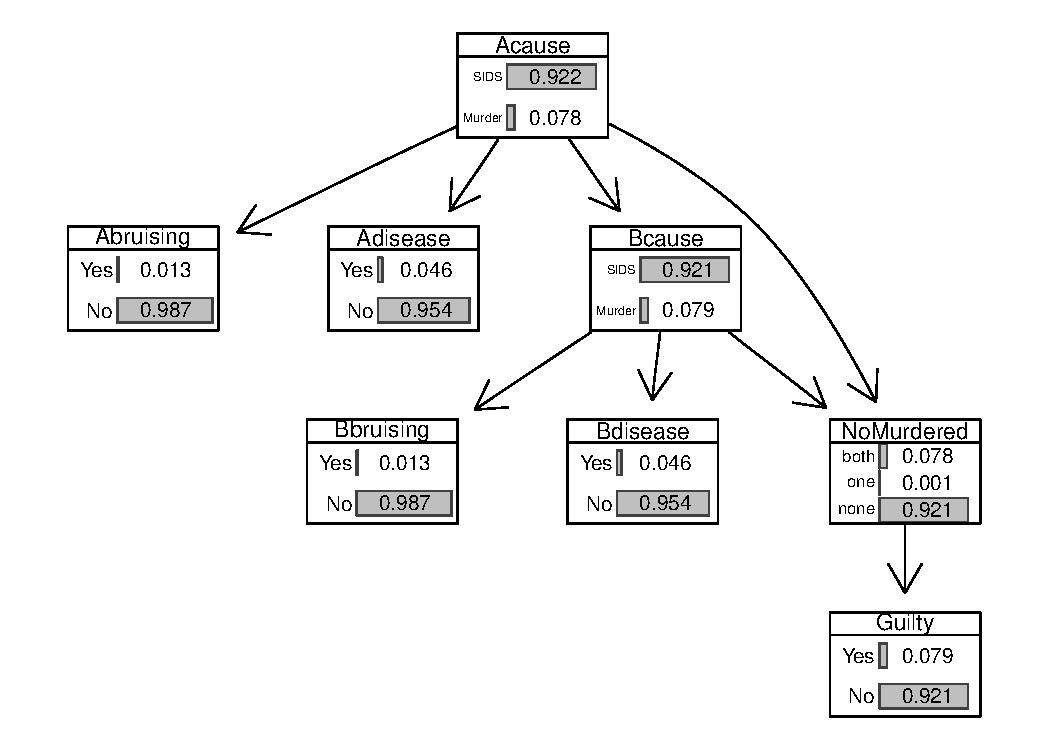
\includegraphics[width=0.7\textwidth,height=\textheight]{imp_philosophical_agust2024_files/figure-pdf/fig-scbnplot-1.pdf}

}

\caption{\label{fig-scbnplot}Bayesian network for the Sally Clark case,
with marginal prior probabilities.}

\end{figure}%

Unfortunately, Bayesian networks, in their standard formulation, inherit
the shortcomings of precise probabilism. The input probabilities should
be precise, but it is often unclear where the values come from or
whether they are justified. Consider the probability that a death by
SIDS would occur. How sure are we that this probability equals 1 in
8,543? Meadow's figure was based on a sample. How big was that sample?
How representative? Other input probabilities need to be entered into
the network to carry out the calculations, for example, the probability
that a mother would kill her children, or the probability that signs of
bruising would be found if Sally was trying to murder her children, and
so on. As they are based on sample frequencies or expert elicitation,
these probabilities will also be uncertain.

The standard response to these concerns is to run a \emph{sensitivity
analysis}: a range of plausible values is tested. Say we are interested
in the output probability that Sally is guilty. The network is updated
by the known facts---the items of evidence---following standard Bayesian
conditionalization. The input probabilities in the network are then
assigned a range of possible values to see how they impact the output
probability of Sally's guilt. Sensitivity analysis is another variant,
perhaps more rudimentary, of imprecise probabilism. In fact, Bayesian
networks for reasoning with intervals and imprecise probabilities
already exist.\footnote{One can use uniform sampling with Bayesian
  networks to approximate the impreciser's commitments
  {[}@caprio2024credal{]}. Another approach is to rely on probabilistic
  programs with the restriction that the variables corresponding to
  probabilities are sampled from uniform distributions corresponding to
  the representor set. A critical survey of approaches along these lines
  shows that, in complex reasoning situations, ``the imprecision of
  inferences increases rapidly as new premises are added to an
  argument'' {[}@KLEITER1996143{]}.} But, as discussed earlier,
imprecise probabilism ignores the shape of the underlying distributions.
It does not distinguish between probability measures in terms of their
plausibility, even though some will be more plausible than others.
Moreover, if the sensitivity analysis is only guided by the values at
the edges of the interval, these extremes will often play an
undeservedly strong role.

These concerns can be addressed by recourse to higher-order
probabilities. In a precise Bayesian network, each node is associated
with a probability table filled in with a finite list of numbers
(precise probabilities). In an imprecise Bayesian network, each node is
associated with a table filled in with an interval of numbers. Instead
of precise numbers or intervals, the probability tables can be filled in
with distributions over the possible first-order
probabilities.\footnote{The densities of interests can then be
  approximated by (1) sampling parameter values from the specified
  distributions, (2) plugging them into the construction of the BN, and
  (3) evaluating the probability of interest in that precise BN. The
  list of the probabilities thus obtained will approximate the density
  of interest.} An example of such a higher-order Bayesian network for
the Sally Clark case can be found in Figure \ref{fig-scwithhop}. This
network helps to assess the impact of the items of evidence on the
ultimate issue, Sally Clark's guilt. The answer is significantly
uncertain even though this might not be apparent by just looking at the
first-order probability of guilt (for details, see
Figure~\ref{fig-scwithhop2}).\footnote{The starting point is the prior
  distribution for the \s{Guilt} node (first graph). Next, the network
  is updated with evidence showing signs of bruising on both children
  (second graph). Next, the assumption that both children lack signs of
  potentially lethal disease is added (third graph). Finally, we
  consider the state of the evidence at the time of the appellate case:
  signs of bruising existed on both children, but signs of lethal
  disease were discovered only in the first child. Interestingly, in the
  strongest case against Sally Clark (third graph), the median of the
  posterior distribution is above .95, but the uncertainty around that
  median is still quite wide. (The lower limit of the 89\% Highest
  Posterior Density Intervals (HPDI) is at .83.)} The upshot is that
relying on precise probabilities only can lead to overconfidence.

\begin{figure}[h]

\centering{

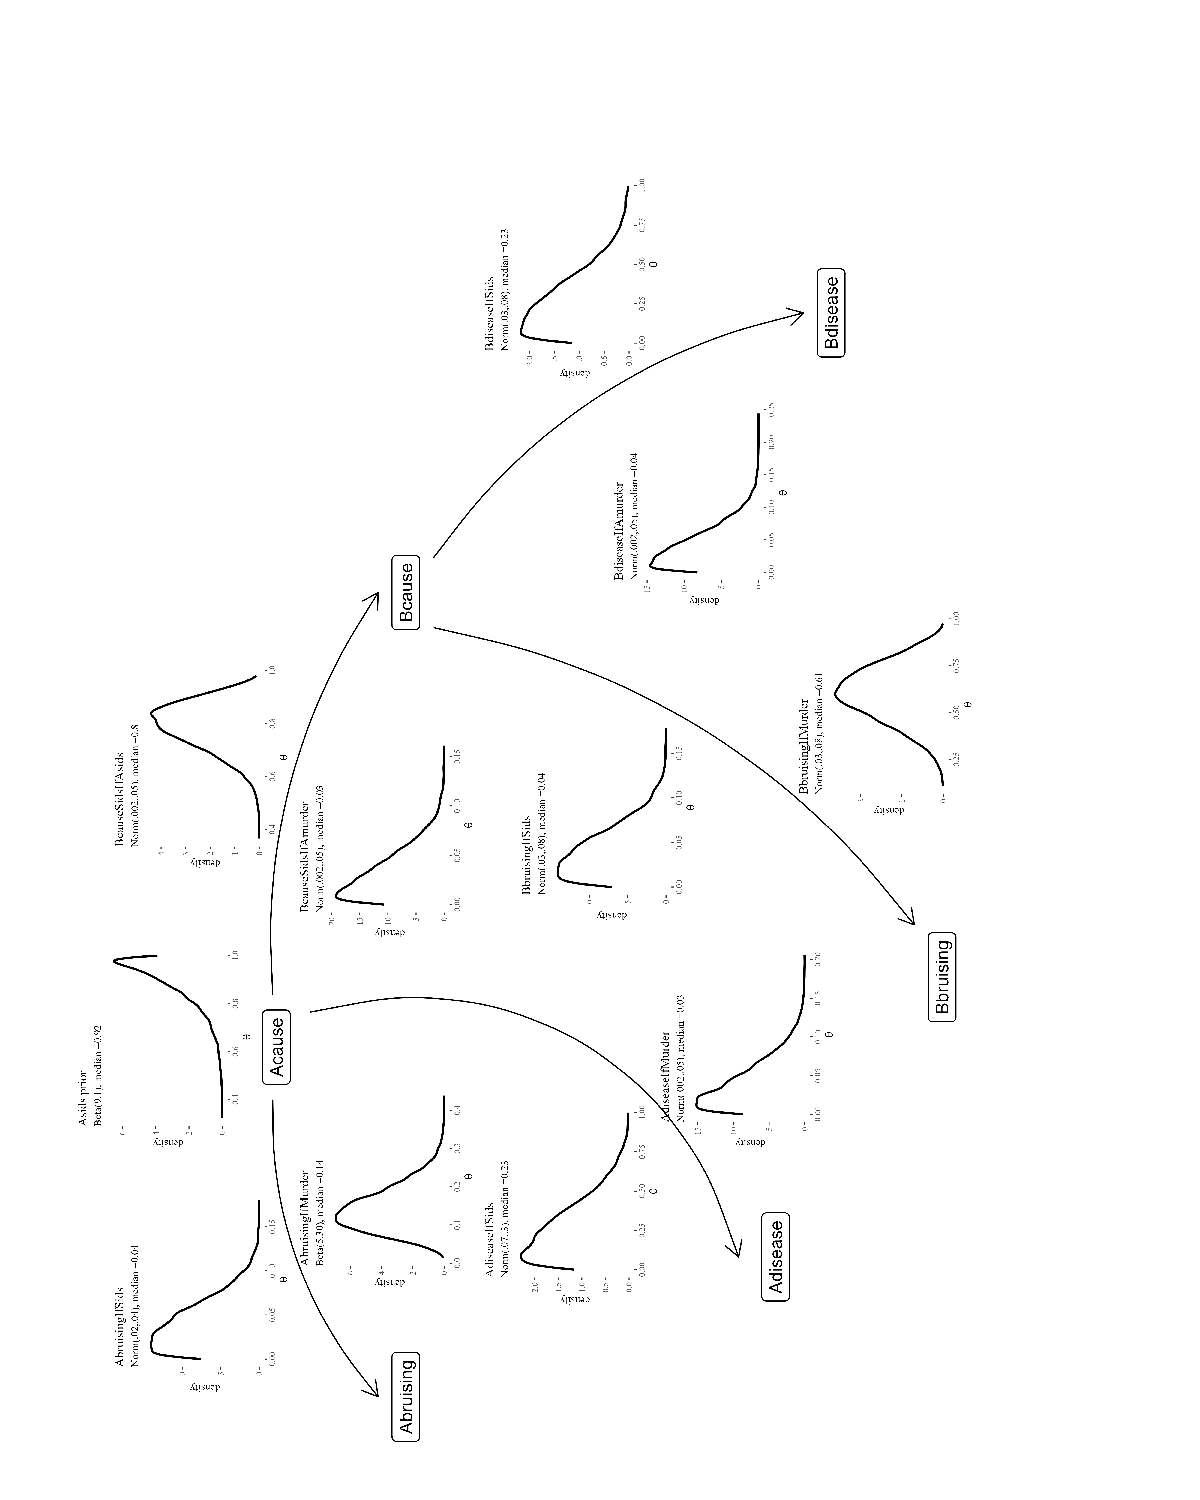
\includegraphics[width=1.2\textwidth,height=\textheight]{rotated_scWithHOPPrint.pdf}

}

\caption{\label{fig-scwithhop}An illustration of a probabilistic program
for the Sally Clark case.}

\end{figure}%

\begin{figure}[H]

\centering{

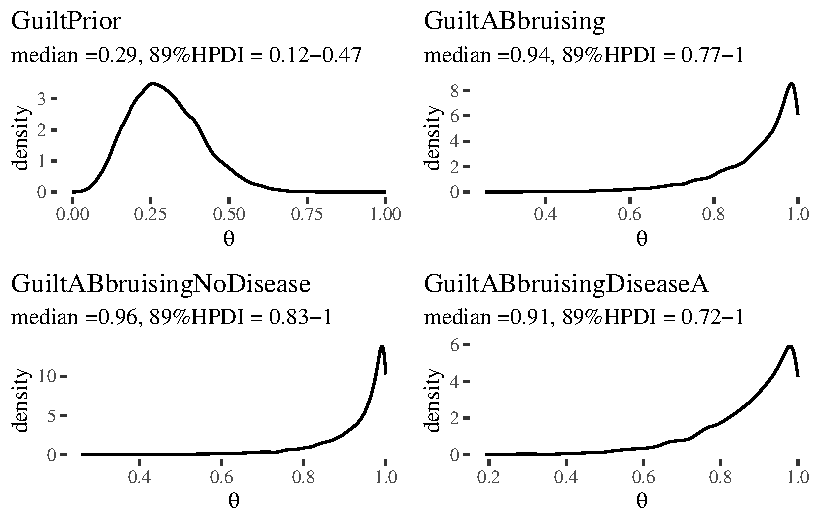
\includegraphics[width=0.7\textwidth,height=\textheight]{imp_philosophical_agust2024_files/figure-pdf/fig-scwithhop2-1.pdf}

}

\caption{\label{fig-scwithhop2}Impact of incoming evidence in the Sally
Clark case.}

\end{figure}%

\section{Conclusion}\label{conclusion}

We have argued that higher-order probabilism outperforms both precise
and imprecise probabilism. It can model scenarios that the other two
cannot model, for example, the case of uneven bias. In addition,
higher-order probabilism does not fall prey to difficulties peculiar to
imprecise probabilism, such as belief inertia and the lack of proper
scoring rules. We have also identified a novel set of problems for
precise and imprecise probabilism, mostly stemming from the question of
how to evaluate, in the aggregate, the probabilities of multiple
propositions. Here again, higher-order probabilism fares better.

Some might dislike the idea of going higher-order for several reasons,
for example, unnecessary complexity. This is a line taken by
@bradley2019imprecise:

\begin{quote}
Why are sets of probabilities the right level to stop the regress at? Why not sets of sets? Why not second-order probabilities? Why not single probability functions? This is something of a pragmatic choice. The further we allow this regress to continue, the harder it is to deal with these belief-representing objects. So let's not go further than we need (pp. 131-132). \end{quote}

\noindent But, given the difficulties of precise and imprecise
probabilism, we are not going further than we need in introducing
higher-order probabilities. The pragmatic concerns are at best unclear.

We should underscore that, mathematically, we do not propose anything
radically new. Concepts from the Bayesian toolkit that can model
higher-order uncertainty already exist. We suggest that they have been
under-appreciated in formal epistemology and should be more widely used.
This is not to say that there is no need for any novel technical work.
One concern is the lack of clear semantics for higher-order
probabilities. While a more elaborate account is beyond the scope of
this paper, the answer should gesture at a modification of the framework
of probabilistic frames
{[}@Dorst2022higher-order;@Dorst2022evidence{]}.\footnote{Start with a
  set of possible worlds \(W\). Suppose you consider a class of
  probability distributions \(D\), a finite list of atomic sentences
  \(q_1, \dots, q_2\) corresponding to subsets of \(W\), and a selection
  of true probability hypotheses \(C\) (think of the latter as
  omniscient distributions, \(C\subseteq D\), but in principle this
  restriction can be dropped if need be). Each possible world \(w\in W\)
  and a proposition \(p\subseteq W\) come with their true probability
  distribution, \(C_{w,p}\in D\) corresponding to the true probability
  of \(p\) in \(w\), and the distribution that the expert assigns to
  \(p\) in \(w\), \(P_{w,p}\in D\). Then, various propositions involving
  distributions can be seen as sets of possible worlds, for instance,
  the proposition that the expert assigns \(d\) to \(p\) is the set of
  worlds \(w\) such that \(P_{w,p}=d\). There is at least one important
  difference between this approach and that developed by Dorst. His
  framework is untyped, which allows for an enlightening discussion of
  the principle of reflection and alternatives to it. In this paper, we
  prefer to keep this complexity side and use an explicitly typed setup.}
Another concern is the lack of an accuracy-based argument in defense of
higher-order probabilism. Will an agent who relies on higher-order
probabilities always accuracy-dominate one who relies on just
first-order probabilities? We leave this as an open question.

\section*{\texorpdfstring{Appendix: the strict propriety of
\(I_{KL}\)}{Appendix: the strict propriety of I\_\{KL\}}}\label{appendix-the-strict-propriety-of-i_kl}
\addcontentsline{toc}{section}{Appendix: the strict propriety of
\(I_{KL}\)}

The fact that \(I_{KL}\) is strictly proper for second-order
probabilities is not very surprising. However, the proof is not usually
explicitly given in the existing literature. We include our argument for
the propriety of \(I_{KL}\) below.

Consider a discretization of the parameter space \([0,1]\) into \(n\)
equally spaced values \(\theta_1, \dots, \theta_n\). For each \(i\) the
`true' second-order distribution if the true parameter indeed is
\(\theta_i\)---we'll call it the indicator of \(\theta_i\)--- which is
defined by \begin{align*}
Ind^k(\theta_i) & = \begin{cases} 1 & \mbox{if } \theta_i = \theta_k\\
                        0 & \mbox{otherwise}  \end{cases}
\end{align*} \noindent We will write \(Ind^k_i\) instead of
\(Ind^k(\theta_i)\). Now consider a probability distribution \(p\) over
this parameter space, assigning probabilities \(p_1, \dots, p_n\) to
\(\theta_1, \dots, \theta_n\) respectively. It is to be evaluated in
terms of inaccuracy from the perspective of a given `true' value
\(\theta_k\). The inaccuracy of \(p\) if \(\theta_k\) is the `true'
value, is the divergence between \(Ind^k\) and \(p\).

\begin{align*}
I_{KL}(p, \theta_k) & = D_\text{KL}(Ind^k||p) \\
& = \sum_{i=1}^n Ind^k_i \left( \log_2 Ind^k_i - \log_2 p_i \right)
\end{align*} For \(j \neq k\) we have \(Ind^k_j = 0\) and so
\(Ind^k_j \left( \log_2 Ind^k_j - \log_2 p_j \right)=0\). Therefore:
\begin{align*}
& = Ind^k_k \left( \log_2 Ind^k_k - \log_2 p_k \right)
\end{align*} Further, \(Ind^k_k= 1\) and therefore
\(\log_2 Ind^k_k =0\), so we simplify: \begin{align*}
& =  - \log_2 p_k
\end{align*}

\noindent Finally, the inaccuracy of a distribution \(q\) as expected by
\(p\), \(\mathit{EI}_{\text{DK}}(p,q)\), is defined as follows:

\begin{align*}
\mathit{EI}_{\text{DK}}(p,q) & = \sum{k =1}^n p_k I_{\text{DK}}(q, \theta_k) \\
& = \sum_{k =1}^n p_k \sum_{i=1}^n Ind^k_i \left( \log_2 Ind^k_i - \log_2 q_i \right)\\
& = \sum_{k =1}^n p_k Ind^k_k \left( \log_2 Ind^k_k - \log_2 q_k \right)\\
& = \sum_{k =1}^n p_k ( - \log_2 q_k) \\
& = - \sum_{k =1}^n p_k \log_2 q_k = H(p,q)\\
\end{align*}

By contrast, the expected inaccuracy of \(p\) from its perspective is
defined as follows:

\begin{align*}
\mathit{EI}_{\text{DK}}(p,p) & = - \sum{k =1}^n p_k \log_2 p_k = H(p)
\end{align*}

Finally, by Gibbs' inequality, \(H(p,q) \geq H(p)\) with identity only
if \(p = q\). So \(I_{\text{DK}}\) is a proper score.

\section{References}\label{references}



\end{document}
